\documentclass[11pt,spanish,a4paper]{article}
% Versión 1er cuat 2014 Víctor Bettachini < bettachini@df.uba.ar >

\usepackage{babel}
\addto\shorthandsspanish{\spanishdeactivate{~<>}}
\usepackage[utf8]{inputenc}
\usepackage{float}
\usepackage{units}
\usepackage{siunitx}
\usepackage{amsmath}
\usepackage{amstext}
\usepackage{amssymb}
\usepackage{graphicx}
\graphicspath{ {./graphs/} {../}}

\voffset-3.5cm
\hoffset-3cm
\setlength{\textwidth}{17.5cm}
\setlength{\textheight}{27cm}

\usepackage{lastpage}
\usepackage{fancyhdr}
\pagestyle{fancyplain}
\fancyhead{}
\fancyfoot{}
\fancyfoot[C]{ {\tiny Actualizado al \today} }
\fancyfoot[RO, LE]{Pág. \thepage/\pageref{LastPage}}
\renewcommand{\headrulewidth}{0pt}
\renewcommand{\footrulewidth}{0pt}


\begin{document}
\begin{center}
	\textsc{\large Física 2 (Físicos)} - Prof. Hernán Grecco\\
	\textsc{\large Primer Cuatrimestre - 2014}\\
	\textsc{\large Guía 9:}	Interferencia
\end{center}

% Michaelson: agregar ejercicio al estilo "agrego un vidrio de espezor". Resaltar la diferencia de camino óptico.

% \emph{LOS EJERCICIOS MARCADOS CON UN ASTERISCO (\textbf{*}) SON OPCIONALES}\\

\begin{enumerate}
	\item Dos ondas planas monocromáticas de igual frecuencia se propagan formando un ángulo \( \alpha \) entre sus vectores de onda.
	Calcule la amplitud e intensidad media en una pantalla perpendicular a la bisectriz entre ambos vectores de onda.


\item Resuelva el problema anterior si las dos ondas son de frecuencia ligeramente diferentes.
	Muestre que la figura de interferencia viaja a lo largo del plano y determine a que	velocidad se mueve.
	Si se desea fotografiar la figura de interferencia, ¿que relación debe haber entre el tiempo de obturación y la diferencia entre ambas frecuencias?
	Si para este experimento se utilizan dos láseres distintos.
	¿Qué longitud de coherencia deben tener como mínimo?
	¿Con cuántas cifras debe estar definida la frecuencia para un caso típico de luz visible?

	
\item Una onda plana incide sobre una lámina de caras paralelas de vidrio de espesor \(d \), con un ángulo de incidencia \(\theta_i \).
	Calcule la amplitud de la onda reflejada teniendo en cuenta solamente las dos reflexiones más intensas.
	Calcule la amplitud de la onda transmitida teniendo en cuenta la que no sufre reflexiones y la que se refleja dos veces.
	Compare la pérdida de energía de la onda transmitida con la energía de la onda reflejada.


\item Se tienen dos fuentes puntuales que emiten en fase ubicadas a una distancia \(d \) entre ellas.
	Calcule la figura de interferencia que se observa en una pantalla ubicada a una distancia \(L \) y perpendicular a la recta de unión entre las fuentes (\(L \gg d \)).
	¿Cómo es la figura en una pantalla paralela a la recta de unión y a una distancia \(L' \) de la misma (\( L' \gg d \))?
	¿Cuántos máximos de interferencia aparecen en cada caso?
	¿Como debe ser la longitud de coherencia para que todos ellos sean visibles?

\item Un \textit{interferómetro de Michelson} es iluminado por medio de una fuente puntual monocromática \(S \).
	Calcule:
	\begin{enumerate}
		\item La posición de los máximos y mínimos en una pantalla ubicada a una distancia \(L \) del divisor de haz.
		\item La posición de los máximos y mínimos en una pantalla ubicada a una distancia \(f \) de una lente de distancia focal \(f \) ubicada a una distancia \(L \) del divisor de haz.
		\item Lo mismo que en \(a \) y \(b \) si se ubica otra fuente \( S' \).
		\item Discuta como se observaría la figura si se ilumina con una fuente extensa.
			Explique porque esta configuración se denomina franjas de igual inclinación.
		\item Indique la expresión de la intensidad que se mide con un detector que detecta el punto central, en función de la diferencia de distancias entre el divisor de haz y los dos espejos.
	\end{enumerate}
	\begin{center}
		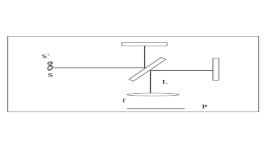
\includegraphics[width=0.3\linewidth]{g09e05}
	\end{center}



\item Un \textit{interferómetro de Michelson} es iluminado por una fuente que emite en dos frecuencias.
	Calcule el valor medio de la intensidad de luz detectada.
	Muestre que cada frecuencia da una contribución sinusoidal con la distancia independiente de las otras frecuencias presentes, y que si multiplica la señal medida por \( \cos{( \omega z/ c)} \) e integra según \(z \) puede recuperar la intensidad de la fuente a la frecuencia \( \omega \).
	¿Cuan largo debe ser el barrido para que la otra frecuencia \( \omega' \) no contribuya?.
	Calcule el caso particular de querer resolver el doblete del sodio.

\item Un \textit{interferómetro de Michelson} permite medir el índice de refracción de gases.
	Una longitud \( L \) del recorrido del haz de uno de sus brazos está ocupada por una celda estanca en la cual se aloja el gas.
	Sus paredes las consideramos transparentes y de espesor despreciable frente a \( L \).
	\begin{enumerate}
		\item En la celda a la que se le ha hecho vacio se inyecta lentamente el gas hasta alcanzar una presión equivalente a la atmosférica (la presión del aire en el otro brazo del interferómetro).
			En el ínterin el patrón de franjas de interferencia cuenta \( N \) nuevas franjas.
			Esto significa que un fotodiodo ubicado en el punto central del patrón proveyó una señal con \( N \) mínimos (o máximos) en función del tiempo.
			Determine el índice de refracción del gas en función de \( n_\mathrm{aire} \), \( \lambda \), \( N \) y \( L \).
	
		\item Se inyecta dióxido de carbono (CO\(_2\)) que a \SI{1}{atm} presenta un índice de refracción \(n= 1.0045 \) en una celda de \(L= \SI{10}{cm} \) iluminando con \( \lambda= \SI{589}{nm}\) provista por una lámpara de sodio (Na).
			¿Cuantas franjas (\( N \)) se registran?
	\end{enumerate}


\item Diseñe (si es posible) un \textit{experimento de Young} a ser realizado por medio de un puntero láser, un papel de aluminio en que perforo dos aberturas muy próximas con un alfiler y observo a ojo desnudo.
	¿Que ventajas tiene utilizar un \textit{biprisma de Fresnel} para realizar el mismo experimento?

	
\item Diseñe un experimento similar al de \textit{Young} pero con dos fuentes sonoras y de modo que ambas orejas caigan dentro de un máximo de interferencia.
	¿Porqué con sonido se pueden usar fuentes independientes?


\item Se realiza un \textit{experimento de Young} utilizando dos aberturas ubicadas a una distancia \(d \) y observando en una pantalla ubicada en el plano focal de una lente colocada delante de las ranuras.
	Discuta que se observa en cada uno de los siguientes casos:
	\begin{enumerate}
		\item Se ilumina las aberturas con una onda plana incidiendo sobre las ranuras con un ángulo \( \alpha \)respecto del eje indicado y en el plano del dibujo.
		\item Se ilumina por medio de una fuente puntual ubicada en el eje.
		\item Se desplaza la fuente puntual fuera del eje.
		\item La fuente no es monocromática sino que tiene una longitud de coherencia de \( 10 \lambda \).
	\end{enumerate}
	\begin{center}
		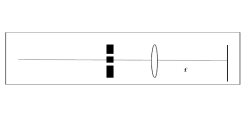
\includegraphics[width=0.25\linewidth]{g09e09}
	\end{center}

	
\item \label{Nfuentes} Se tienen N fuentes puntuales monocromáticas en línea equiespaciadas.
	Calcule las	franjas de igual inclinación si se observa a lo largo del eje determinado por las fuentes.
	Calcule el ancho de las franjas claras y la separación entre ellas.
	¿Qué se observa a lo largo del eje de las fuentes en función de la separación entre las fuentes?
	¿Cómo cambia con el número de fuentes?
	Si las fuentes emiten en dos colores, ¿en qué condiciones quedan separados nítidamente los respectivos máximos?


\item Repita el problema anterior observando a lo largo de un eje perpendicular a las fuentes.
	¿Qué se observa ahora que cambia con la separación entre fuentes y con el número de fuentes?


\item  Resuelva el problema de la lámina de caras paralelas con incidencia normal a las caras asumiendo una solución autoconsistente en vez de hacer una suma infinita: considere que dentro de la lámina hay una onda hacia la derecha \( \Psi_3 \) y otra hacia la izquierda \( \Psi_4 \), que incide una onda de la izquierda \( \Psi_1 \), se refleja una onda hacia la derecha \( \Psi_2 \) y se transmite una onda \( \Psi_5 \).
	Resuelva las incógnitas planteando las condiciones de borde (reflectividad y transmisión en cada cara).
	\begin{center}
		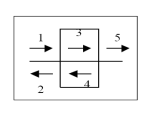
\includegraphics[width=0.15\linewidth]{g09e13}
	\end{center}


\item Resuelva nuevamente el caso de la lámina de caras paralelas teniendo en cuenta ahora las infinitas reflexiones.


\item Compare la solución del \textit{interferómetro Fabry-Perot} con la solución del problema \ref{Nfuentes}.
	¿En que se parecen y en que difieren? ¿Quien juega el papel de la distancia entre fuentes y cual es el número de fuentes equivalentes que da los mismos anchos característicos de los máximos?

\end{enumerate}
\end{document}
